% REMEMBER: You must not plagiarise anything in your report. Be extremely careful.

\documentclass{l4proj}

    
%
% put any additional packages here
%

\begin{document}

%==============================================================================
%% METADATA
\title{A Seamful Game Based on GPS Shadows}
\author{Robbert Malcolm Sinclair}
\date{14 October 2022}

\maketitle

%==============================================================================
%% ABSTRACT
\begin{abstract}
    Every abstract follows a similar pattern. Motivate; set aims; describe work; explain results.
    \vskip 0.5em
    ``XYZ is bad. This project investigated ABC to determine if it was better. 
    ABC used XXX and YYY to implement ZZZ. This is particularly interesting as XXX and YYY have
    never been used together. It was found that  
    ABC was 20\% better than XYZ, though it caused rabies in half of subjects.''
\end{abstract}

%==============================================================================

% EDUCATION REUSE CONSENT FORM
% If you consent to your project being shown to future students for educational purposes
% then insert your name and the date below to  sign the education use form that appears in the front of the document. 
% You must explicitly give consent if you wish to do so.
% If you sign, your project may be included in the Hall of Fame if it scores particularly highly.
%
% Please note that you are under no obligation to sign 
% this declaration, but doing so would help future students.
%
\def\consentname {Robbert Malcolm Sinclair} % your full name
\def\consentdate {14 October 2022} % the date you agree
%
\educationalconsent


%==============================================================================
\tableofcontents

%==============================================================================
%% Notes on formatting
%==============================================================================
% The first page, abstract and table of contents are numbered using Roman numerals and are not
% included in the page count. 
%
% From now on pages are numbered
% using Arabic numerals. Therefore, immediately after the first call to \chapter we need the call
% \pagenumbering{arabic} and this should be called once only in the document. 
%
% Do not alter the bibliography style.
%
% The first Chapter should then be on page 1. You are allowed 40 pages for a 40 credit project and 30 pages for a 
% 20 credit report. This includes everything numbered in Arabic numerals (excluding front matter) up
% to but excluding the appendices and bibliography.
%
% You must not alter text size (it is currently 10pt) or alter margins or spacing.
%
%
%==================================================================================================================================
%
% IMPORTANT
% The chapter headings here are **suggestions**. You don't have to follow this model if
% it doesn't fit your project. Every project should have an introduction and conclusion,
% however. 
%
%==================================================================================================================================
\chapter{Introduction}

% reset page numbering. Don't remove this!
\pagenumbering{arabic} 


Why should the reader care about what are you doing and what are you actually doing?
\section{Guidance}

\textbf{Motivate} first, then state the general problem clearly. 

\section{Writing guidance}
\subsection{Who is the reader?}

This is the key question for any writing. Your reader:

\begin{itemize}
    \item
    is a trained computer scientist: \emph{don't explain basics}.
    \item
    has limited time: \emph{keep on topic}.
    \item
    has no idea why anyone would want to do this: \emph{motivate clearly}
    \item
    might not know \emph{anything} about your project in particular:
    \emph{explain your project}.
    \item
    but might know precise details and check them: \emph{be precise and
    strive for accuracy.}
    \item
    doesn't know or care about you: \emph{personal discussions are
    irrelevant}.
\end{itemize}

Remember, you will be marked by your supervisor and one or more members
of staff. You might also have your project read by a prize-awarding
committee or possibly a future employer. Bear that in mind.

\subsection{References and style guides}
There are many style guides on good English writing. You don't need to
read these, but they will improve how you write.

\begin{itemize}
    \item
    \emph{How to write a great research paper} \cite{Pey17} (\textbf{recommended}, even though you aren't writing a research paper)
    \item
    \emph{How to Write with Style} \cite{Von80}. Short and easy to read. Available online.
    \item
    \emph{Style: The Basics of Clarity and Grace} \cite{Wil09} A very popular modern English style guide.
    \item
    \emph{Politics and the English Language} \cite{Orw68}  A famous essay on effective, clear writing in English.
    \item
    \emph{The Elements of Style} \cite{StrWhi07} Outdated, and American, but a classic.
    \item
    \emph{The Sense of Style} \cite{Pin15} Excellent, though quite in-depth.
\end{itemize}

\subsubsection{Citation styles}

\begin{itemize}
\item If you are referring to a reference as a noun, then cite it as: ``\citet{Orw68} discusses the role of language in political thought.''
\item If you are referring implicitly to references, use: ``There are many good books on writing \citep{Orw68, Wil09, Pin15}.''
\end{itemize}

There is a complete guide on good citation practice by Peter Coxhead available here: \url{http://www.cs.bham.ac.uk/~pxc/refs/index.html}. 
If you are unsure about how to cite online sources, please see this guide: \url{https://student.unsw.edu.au/how-do-i-cite-electronic-sources}.

\subsection{Plagiarism warning}

\begin{highlight_title}{WARNING}
    
    If you include material from other sources without full and correct attribution, you are commiting plagiarism. The penalties for plagiarism are severe.
    Quote any included text and cite it correctly. Cite all images, figures, etc. clearly in the caption of the figure.
\end{highlight_title}


%==================================================================================================================================
\chapter{Background}

In this chapter I will go over some of the foundational concepts required to understnad the background of the project

\section{Introduction to the Global Positioning System (GPS)}

The Global Positioning System also known as GPS is one of the worlds most famous Global Navigation Satellite Systems (GNSS). It allows people to determine their
location from anywhere around the world at any time. GPS has three main phases, the space phase, the control phase and the user phase.
In the space phase, the earth is split up into 24 "slots" which should be filled up by an operational satellite \citep{spsStandard}. Therefore
the GPS constellation is made up of at least 24 opterational satellites. In an ideal situation a user should have access to at least 4 of the satellites
at any one time \citep{Rabbany2006}. 

Each GPS satellite consistently sends down radio signals down to the Earth's surface. As of 2020 there are three main frequencies
these are L1 which emits at 1575.42 MHz, L2 which emits radio waves at 1227.6 MHz and L5 with 1176.45 MHz \citep{spsStandard}. This project
will most likely be using L2 and L1 as L5 is used mainly for aviation safety \citep{Xu2016} A GPS receiver will pick up this data and can use the clock signals to calculate the distance from each satellite. Once a 
satellite distance is calculated we can create a radius of equidistant points. We can then add the signals from several other
satellites to find the intersection points. We usually need 3 to 4 satellites to be able to pinpoint the GPS receiver on the map. \citep{Rabbany2006}



%TODO - Add a source and paragraph about how GPS is calculated

\section{What causes Inaccuracies in GPS Systems}
In this project we will be looking at making a game based on GPS shadows which are areas where the GPS signal is not as accurate. In this section I will look
at the various factors that could effect our accuracy.

\subsection{GPS Clock Errors}
% ROUGH DRAFT - Rewrite this with proper sources when you've found them

The first form of GPS error is a clock error. Each satellite sends signals down using an atomic clock which while accurate, can still have a 
slight delay. This delay will be small (a few nanoseconds long) but will accumulate over time. One of the main reasons why this can lead to
a decrease in accuracy is that the receiver may get a time on the clock which is off the actual time on the satellites clock. This can lead to
a slight change of position. This form of error is common with most GPS signals. A typical GPS Receiver can also be a cause for this problem as it 
has a crystal clock which is not as precise than the cesium atomic clocks on the satellites \citep{Rabbany2006, Kleusberg1990}. While this
form of error is a common cause of problem with GPS accuracy, there aren't a lot of game opportunities due to the fact that the player
can't really control when a clock error is to happen.

\subsection{GPS Signal Reception}
GPS signals are in the form of radio waves which can be blocked by obstacles on the way to a GPS sensor. When signals hit a specific obstable
the signals decrese in quality during a process known as attenuation \citep{Indoor2010}. Some examples of such obstacles include
building walls, soil and water. \citep{Kleusberg1990}. Eventually the GNSS receiver will receive more noise
than the original signal which leads to an inaccurate signal. A good signal is received when the receiver has a good signal from at least 4
satellites. Therefore in urban areas with high rise buildings, one or more satellites could be obstructed. If a game was to be made
using this concept then the game would be best played in dense urban areas.

\section{Seamful Design}


\section{Guidance}
\begin{itemize}    
    \item
      Don't give a laundry list of references.
    \item
      Tie everything you say to your problem.
    \item
      Present an argument.
    \item Think critically; weigh up the contribution of the background and put it in context.    
    \item
      \textbf{Don't write a tutorial}; provide background and cite
      references for further information.
\end{itemize}

%==================================================================================================================================
\chapter{Analysis/Requirements}
In this section I go over the main process that I used to come up with a design for the game

\section{Creating an app to get GPS locations}
Since I didn't have much knowledge of mobile app development. I gathered that the best place to start was to make an app that gets a location. 
I started by doing some research into creating an Android app using Kotlin. The main aim of this app was to get me the latitude and longitude coordinates every second and most importantly, give me the accuracy for the GPS locations. 
In order to get this up and running quickly, I tested two main GeoLocation APIs, the FusedLocationProvider API and the LocationManger which can be found in the Android Documentation.

\subsection{FusedLocationProvider API}
The first API I tried was the FusedLocationProvider API as this was the first one that I found. The FusedLocationProvider API combines both GPS and WiFi geolocation
techniques to try and create an optimal location \citep{fused}. This API allowed me to create a basic location app quickly so that I could start finding GPS locations
within my local area. As figure \ref{fig:fusedhist} shows, the location data that I gathered was skewed towards values with an accuracy of less than 50. While a lot of
points were under the 20 meters area. However as you can see, there was a decent amount of values above 50 meters meaning that the API picked up a lot of shadows.
This API would have been a good one to use for my game as I would have had a lot of shadow areas for a player to hide. However the main flaw was that
it was giving me a combination of both Wifi and GPS coordinates. Thies meant that I was more likely to find shadows in areas with low WiFi. This would
explain why I had a lot of shadow areas when I walked around Kelvingrove Park, an area which I thought would have a very accurate signal due to the lack of buildings.

\begin{figure}
    \centering
    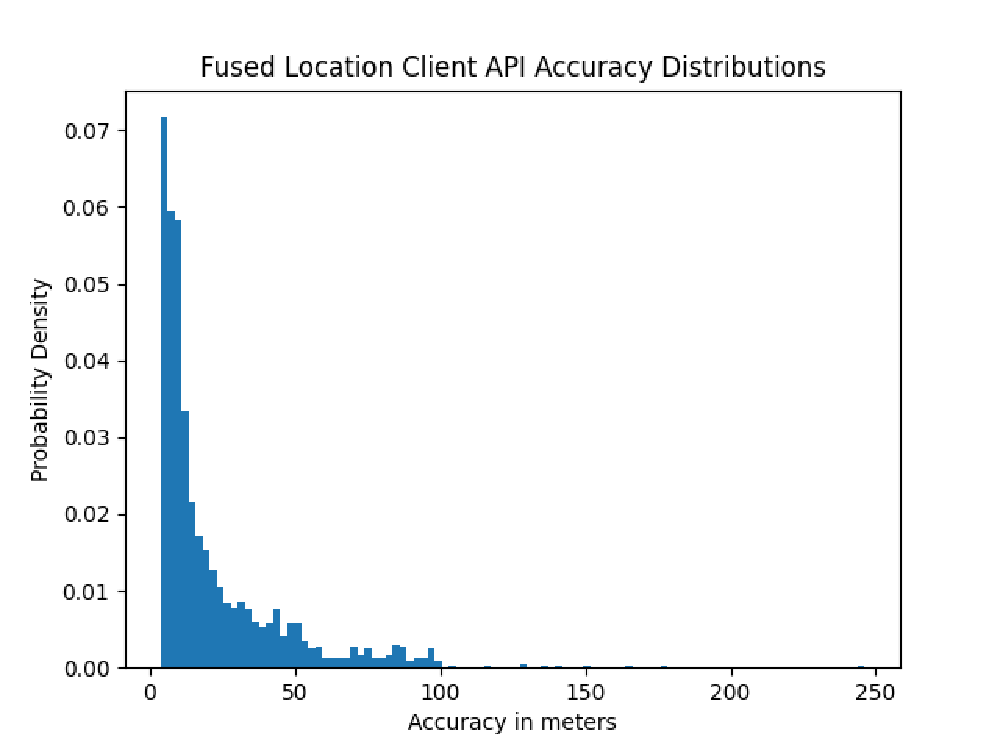
\includegraphics[width=0.6\linewidth]{images/fused_histogram.pdf}    

    \caption{Histogram showing the ranges of accuracy (in meters) of location points picked up by the FusedLocationProvider API}

    % use the notation fig:name to cross reference a figure
    \label{fig:fusedhist} 
\end{figure}

\subsection{LocationManger API}
\label{locationManager}
Since the FusedLocationProvider wasn't appropriate for the project, I needed to find an API that would give me location data based purely on GPS. One of the libraries that I found
from the Android Developers Website was the "LocationManger" API. The LocationManager API gives me more control over what kind of Geolocation I was getting on my phone. Therefore
I was able to ensure that my geolocation was based on a full GNSS navigation system. \citep{locationManager} The other main advantage to this library is that with the use of the "requestLocationUpdates" method and
the "LocationListener" interface, I can easily control what my app does when it receives a new location.

While there are some advantages to using the LocationManager API, it does come with some disadvantages as well. For one thing, there are significantly less shadow areas when using
pure GNSS coordinates. The only real areas where there are major shadows are within buildins, under bridges or in enclosed areas. This is because on my phone, it can track up to 
15 satellites when getting my location. In comparison to figure \ref{fig:fusedhist}, figure \ref{fig:mongohist} shows that there is one big peak in the overall accuracy of all the spots.
When walking around with my app I noticed that for most of the time, my accuracy was 3.795 meters of accuracy. However while at first glance this may be a disadvantage the main advantage for creating a
game is that compared to the Fused Location API. It is better overall for an overall game design because the areas where shadows can be found will be more consistent than the ones
found in the Fused Location API. Therefore the game can be used to teach people where GPS can decrease in quality.

\begin{figure}
    \centering
    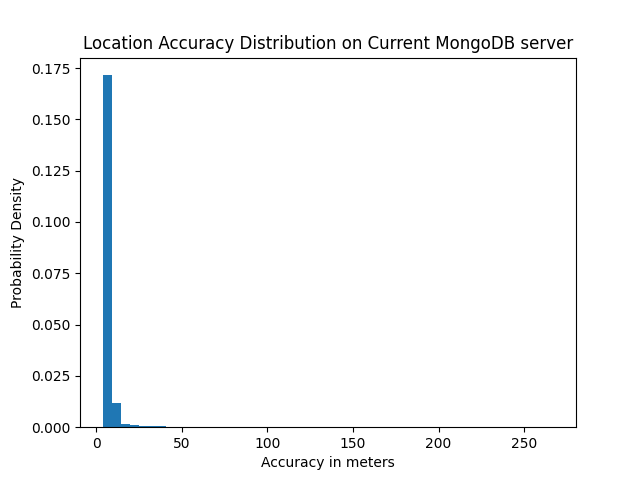
\includegraphics[width=0.6\linewidth]{images/mongo_db_histogram.png}

    \caption{Histogram showing the ranges of accuracy (in meters) of location points picked up by the LocaitonManager API}

    \label{fig:mongohist}
\end{figure}

\section{Guidance}
Make it clear how you derived the constrained form of your problem via a clear and logical process. 

%==================================================================================================================================
\chapter{Design}
How is this problem to be approached, without reference to specific implementation details? 
\section{Guidance}
Design should cover the abstract design in such a way that someone else might be able to do what you did, but with a different language or library or tool.

\section{Overview}
\label{game-overview}
The game that I will make is a simple tag game where a player can take advantage of GPS shadows in order to hide from
the chaser. The chaser will be able to see the other users locations in real time if the runner is in an area with
high GPS accuracy. Once a chaser tags a runner, the caught runner becomes the chaser and a 30 second Jail Time is
triggered. During this time the catcher cannot see the runner's latest location or is able to catch a runner.

The game will have a time limit with the first iteration being 15 minutes. This is so that the game can be quick and
easy to play during a study break. I also considered the fact that the game would work well in dense urban environments
with lots of buildings to go into like the University of Glasgow campus. Once the time limit is up, the winner will
be calculated as the person who was the runner for the most amount of time in total.

\section{Architecture}
The game that I will create will utilise a Client-Server Architecture. The client will be a smartphone with a GPS or
GNSS sensor. Several clients will be connected using a WebSocket. The smartphone will get the GNSS data including the
latitude, longitude and accuracy and then will process it and send to the server. The location data will also be sent 
to the UI where the user's overall position will be updated. Through the websocket, the phone will send the GPS data
to the server which will save the users location onto a geospatial database. Depending on certain conditions, the data
will be sent to the rest of the clients.

\subsection{Client (Smartphone)}
\label{designClient}
The smartphone app will be divided into four main components. These are the GPS Listener, the Communications area, the
Player and the User Interface. When the client first connects to the server, it will give the user a player id and a player
type. This information will be given to the player class which stores the id for any further communications with the server.
Then once that is done, the GPS Listener will start to fetch the GPS coordinates every 2 seconds. This data is then sent
to the User Interface so that the map is updated with the user's location. The GPS coordinates are then sent to the Communication
class where they are sent to the server.

\subsection{Server}


\subsection{Client Server Communication}
\label{communication}
Since a lot of the game will have a lot of multiplayer features, it was important that the network side of the game
was robust to ensure that no player would have an unfair advantage when playing the game. Table \ref{tab:webSocketComms}
sets out the different communication types that are required to make this game.

\begin{table}[]
    \caption{The different communication types to the server  }\label{tab:webSocketComms}
    \resizebox{\textwidth}{!}{\begin{tabular}{|l|l|}
    \hline
    \rowcolor[HTML]{9B9B9B} 
    \multicolumn{1}{|c|}{\textbf{Communication Type}} & \multicolumn{1}{c|}{\textbf{Method and Purpose}}                                             \\ \hline
    CONNECT               & Gives the user their id and their initial player type                                                                \\ \hline
    NEW\_TYPE             & This is triggered if either a new user connects to the server or if a user is caught. This will change the users type \\ \hline
                          &                                                                                                                      \\ \hline
    \end{tabular}}
    
    \end{table}

\section{Mechanics}
In this section I go over the various mechanics that I have designed for the game

\subsection{Player Types}
When the player joins the game, they will be assigned to one of two player types. These are the "Chaser" or the "Runner".
The role of the Chaser is to catch a runner as described in section \ref{catching}. When the catcher does this they give the role of chaser to the runner. The Chaser
will be able to see the real time locations of any runner in the game.

The goal of a Runner is to avoid being caught by the Chaser as mentioned before. The Runner will not have a real time
view of the Chaser but will have the ability to "hide" from them by going into areas with a low GPS density. If their
GPS accuracy is low enough, they will not transmit their location to the chaser. Making them invisible to the chaser.
The Runners will also not transmit any location data during the jail period as mentioned in section \ref{game-overview}.

In previous iterations of my design the Runner would have been able to have seen all of the GPS Shadows within a 50
meter radius. The Shadows would be small red dots on the users maps. However after implementing this feature the screen
would freeze up leading to a poor user experience and it gave the Chaser an unfair advantage as they didn't get any
performance issues with just the Runner locations on the screen.

\subsection{Location Tracking and Catching}
\label{catching}
As mentioned before, both the runner and the chaser transmit data to the server. After a set interval
the latest latitude and longitude coordinates will be sent to the server which will update the player's location
in the database. Once this data is collected the chaser is then able to determine if they have caught a runner.

The chaser will have a 5 meter "no-go zone" which will be the way to determine if a player is caught or not. If
the GPS accuracy is high and a player has entered the Chaser's 5 meter radius, then the runner is considered to be 
"caught". My original idea was to calculate the distance on the smartphone however I realised that the main disadvantages
to this was that it was going to be difficult to track who the chaser was. I also thought that since the main architecture
was a Client-Server system that going for as thin a client as possible would be the best approach due to the computational
limitations of a smartphone.

\subsubsection{Phase 2 Design}
During my Phase 1 evaluation I noticed that the design mentined in section \ref{catching} was not as suitable due to 
multipath errors(see section \ref{phase1catching} for more details). The main problem being that if the catcher tried
to catch a player, they would have to move around before it would register. For phase 2 I will make a more dynamic design
where the catch radius will increase or decrease depending on how likely a multipath error was able to occur. Uber found
a way to improve their GPS accuracy by making use of the signal noise ratio of each satellite and comparing it to a 3D map.
They found that a high ratio would mean that the sensor is in direct view of a satellite while a low satellite would mean that
the signals were more likely to be obstructed by buildings, trees and other obstables \citep{uberGPS}. While using a 3D map
to improve the catching mechanic is out of the scope for the project, I will take the idea of getting the average SNR. I will
now dynamically increase and decrease the catch radius by dividing 5 from the average ratio (as a number between 0 and 1). My hope
is that if two players are closer together, a catch will be more likely to be registered.
%==================================================================================================================================
\chapter{Implementation}

\section{Process}
\label{process}
The game was developed using an iterative approach where I took the time to design some game mechanics, implement them and
then evaluate it with other users. This has helped me when designing the core mechanics of the game and it has allowed me
to see what other people would want in future iterations.

\section{Technologies Used}

\subsection{Server}
\label{implementationServer}
When designing my system, I knew early on that I needed to set up a server in order to keep track of people's location
and to give the user updates on who is playing or not. To do this I needed a server side framework that would make real
time communication easier and that would allow me to easily implement a WebSocket. Initially I made a Django server to
handle the requests making use of the Django Channels library. However this proved difficult when deploying the application.
This was because in order to use Django with a WebSocket you need to configure it with ASGI rather than the default WSGI
to allow for asynchronous communication. This proved to be rather difficult, therefore I decided to abandon Django for this
project.

The final version of the server is written using Node.js. The main reason why I decided to migrate to this technology is that
I could easily set up what I needed without worrying about all of the extra stuff that I would need to implement if I where to
stick to Django. It also had an easier WebSocket library \emph{ws} which allowed me to develop my communication system quickly
and effectively. Another benefit to using Node.js was that I could use any database that I wanted meaning that I could
choose the right one for the job. If I were to have stayed with Django I would have been limited to popular SQL databases
such as PostGreSql, Oracle or MySQL \citep{djangoDatabases}. Node.js allows me to be more flexible and it's light weight
design means that I can make the server side code as big or as small as I need it to be.

\subsection{Database}
As I mentioned in section \ref{implementationServer}, the freedom of using Node.js meant that I could really have a look
around for suitable databases. Since the design of the catching mechanic was that the chaser had a no-go radius (see section
\ref{catching} for more details), I decided that I wanted to use a database which had the potential to have Geospatial queries.
Two of the most popular databases that would allow me to do that would be PostGIS which is a modified version of PostGreSql \citep{postgis, postgres} and
MongoDB which is a popular document based database \citep{mongodb}. In the end I decided to go with MongoDB since their API
was easy to use and implement. With MongoDB I could use their GeoSpatial Processing with minimal setup. Also it is significantly
faster than PostGIS in processing proximity queries \citep{Bartoszewski2019}. This was especially important considering
that I would be querying this database every time another player broadcasts their location.

\subsection{Mobile App}
As mentioned in section \ref{designClient}, the client will interact with the game through a mobile app. After a lengthy
analysis of different programming languages and frameworks that I could use, I finally settled on making a native Android
app using the Kotlin programming language \citep{kotlin}. I chose to write my code in Koltin because it has a simple syntax
and is now the recommended language for building android apps by Google. It also contains UI libraries such as Jetpack Compose 
which makes UI design and implementation easy to implement.

Another main reason why I went for Koltin is that other cross-platform mobile frameworks did not have the APIs required
to get pure GNSS coordinates. Kotlin has the LocationManager API (See section \ref{locationManager}) which allows me
to gain GNSS coordinates and some vital information like the signal noise ratio (SNR) of each satellite \citep{locationManager}
which gives me a lot of further information which can be useful for creating algorithms that can determine whether a player
is in a GPS Shadow or not.

\subsection{Deployment}
\label{deployment}
Having the front-end of the game as a Kotlin app brought a couple of challenges when developing. For one thing, it meant
that I couldn't run my server locally if I wanted to test my location tracking or other features with my mobile app. Therefore
I needed to find a hosting service that would allow me to deploy quickly and with very little effort. Railway.app \citep{railway}
is a cloud base deployment service that auto deploys after every git commit. Since I had a GitHub repository, it meant that it was
easy to deploy my code onto a server. Therefore I could focus more on the overall development rather than how to get it on a server.

\section{Mobile Side}

\subsection{User Interface}
\label{implementationui}

\begin{figure}
    \label{fig:ui_imp}
    \centering
    \begin{subfigure}[b]{0.45\textwidth}
        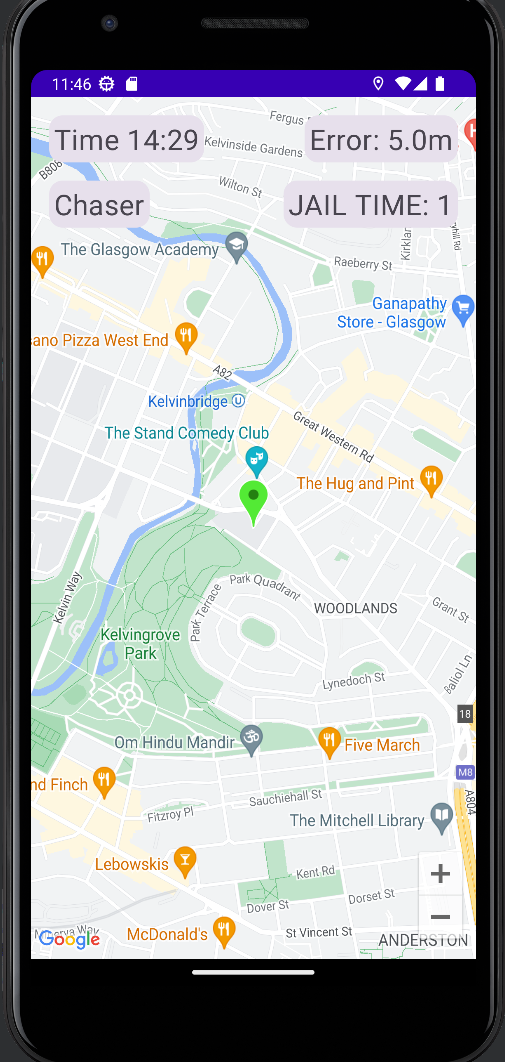
\includegraphics[width=\textwidth]{images/ui_chaser.png}
        \caption{The Chaser view.}
        \label{fig:ui_chaser}
    \end{subfigure}
    ~ %add desired spacing between images, e. g. ~, \quad, \qquad, \hfill etc. 
      %(or a blank line to force the subfigure onto a new line)
    \begin{subfigure}[b]{0.45\textwidth}
        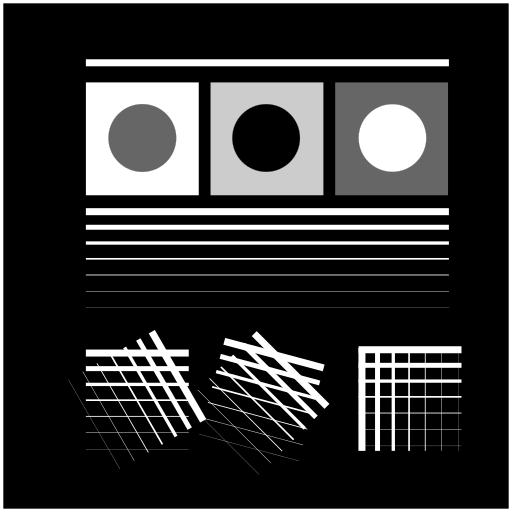
\includegraphics[width=\textwidth]{images/synthetic_2.png}
        \caption{The Runner View}
        \label{fig:ui_runner}
    \end{subfigure}
    
    \caption{These two screenshots show the runner and the chaser states that the players
    will see when playing the game. \ref{fig:ui_chaser} shows you what a chaser player would
    see while the game is in progress while \ref{fig:ui_runner} shows you what a runner would
    be able to see.
    }
\end{figure}
For the game to be accessible to users I needed to make a User Interface that was
clear and simple to use for the duration of the game. Figures \ref{fig:ui_chaser} and \ref{fig:ui_runner} 
gives you a view of the two different screens that the player would get when they start a
game. The final design takes advantage of the Google Maps SDK for Android which has
an easy to use API for working with maps with Jetpack Compose \citep{GoogleMaps}.

The UI features at the top of the app are the same for both player types. On the top
left corner, the player has a view of how long they have left in the game, the timer
counts down from 15 minutes and is synced with the server time every 30 seconds to 
ensure that every player has the correct time. The top right of the UI gives the
user's GNSS error to 1 decimal places. This will give the user feedback on whether
their location is a good hiding spot or not. Finally the last row includes a label
to tell the player what type of player. To the right of that label is the "Jail Time"
label which only shows in the 30 seconds after a player is caught or when the game is
started.

As seen in figure \ref{fig:ui_chaser}, the Chaser view doesn't have a lot of extra features
compared to the runner view. The only main difference is that there is a marker to show the
runners locations. In both player types, the player's current location is marked in green and
all other players will have a red marker. This is in response to feedback from phase 1 (see section
\ref{phase1survey} for more discussion on this) as in that phase I had markers which were the same
colour.

The Runner User Interface (Shown in figure \ref{fig:ui_runner}) has one key exclusive feature. This is the see Chaser button. If the user
is in a high GPS location for a full minute, they will be able to press the "See the Chaser" button
at the bottom of the screen. This will give the user a 3 second view of the chaser's location. This
was another addition in response to feedback from the evaluation in phase 1.

\section{Server Side}
\label{serverside_imp}

\subsection{Overview}
\label{serverOverview}
The server side code of the game had to handle multiple different types of WebSocket messages and it needed
to be able to query my MongoDB database. Figure \ref{fig:serverSideOverview} shows the general architecture
on the server side. When the user connects to the game, the requests using the HTTP and WebSocket requests
are handled by index.js. Most of the other configuration is handled here, for example instances of the classes
defined in GPSMongo.js and GameLog.js are initialized here. Once the user has successfully connected to a WebSocket,
any further messages are processed in WebSocketOperations.js. Depending on the event required the data is sent
to GPSMongo.js or GameLog.js which then queries one of three collections (GPSShadows, players, games) in my MongoDB database.

\subsection{WebSocketOperations.js}
As I mentioned in section \ref{serverOverview}, the WebSocketOperations.js file is the main base of operations for
the rest of the game. Whenever a user connects to a server, the methods inside the WebSocketOperations class will take
the user's details like their phone brand and model and then returns them with an id. This id is attached to the connection
object that I could use to keep track of which player is sending the message. The WebSocketOperations.js file is also
responsible for keeping track of whether a game is running or not. If the user were to press the start game button on the
user interface, then the class will run the various methods to work out who will be the chaser.

While the game is running, the WebSocketOperations class will also do some background tasks to make sure that no
player would have an unfair disadvantage while playing the game. The most important task is to have time sync for
the overall game time and when a player ends their jail time. This works by having a background asynchronous method
that counts out 30 seconds. When that time is up, the server will broadcast the current time to all of the players.
I thought that this was necessary due to the fact that while I had a working timer on the User Interface, I would
notice that the times would get out of sync with the other players. I also wanted to ensure that both the jail time
and the game as a whole would end for both players at the same time to avoid any problems or glitches that could happen
if one player was still in the game and another was outside the game. The server allowed me to address any syncing
problems on the mobile app.

As well as keeping the time of the game, the WebSocketOperations.js file has a lot of other systems in place for enforcing the
rules of the game. One of the main parts of my design for the game was that a Chaser would not be allowed to see the Runner's
location if the game was in Jail Time or whether the player was in a Shadow. I managed to implement this rule by making
a function within this file that executes whenever a phone sends a location object. This was especially useful as I could
use it to ensure that locations would always go to the logging database, but will only go to the chaser player if a certain
condition was met.

\subsection{GPSMongo.js and GameLog.js}

\subsection{The MongoDB collections}


\begin{figure}
    \centering
    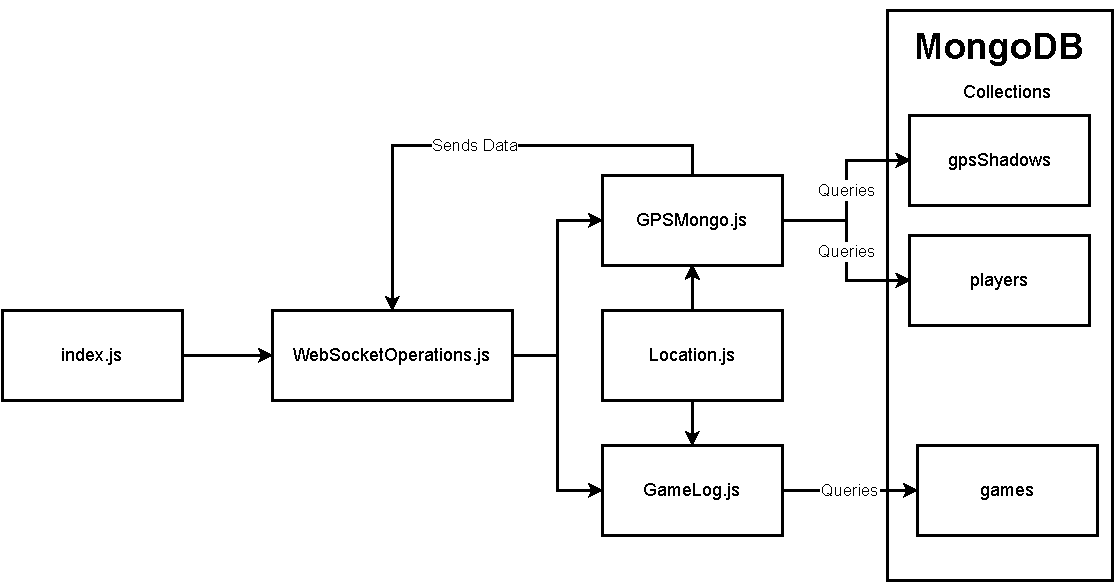
\includegraphics[width=\linewidth]{images/serverSideOverview.pdf}    

    \caption{
        The diagram shows the main flow of files from the server. All requests start at index.js which are
        then processed by the WebSocketOperations.js file. This file will call methods in either the GPSMongo
        and GameLogMongo.js files which make the queries to the MongoDB database.  
    }

    % use the notation fig:name to cross reference a figure
    \label{fig:serverSideOverview} 
\end{figure}



\section{Guidance}
You can't talk about everything. Cover the high level first, then cover important, relevant or impressive details.



\section{General points}

These points apply to the whole dissertation, not just this chapter.



\subsection{Figures}
\emph{Always} refer to figures included, like Figure \ref{fig:relu}, in the body of the text. Include full, explanatory captions and make sure the figures look good on the page.
You may include multiple figures in one float, as in Figure \ref{fig:synthetic}, using \texttt{subcaption}, which is enabled in the template.



% Figures are important. Use them well.
\begin{figure}
    \centering
    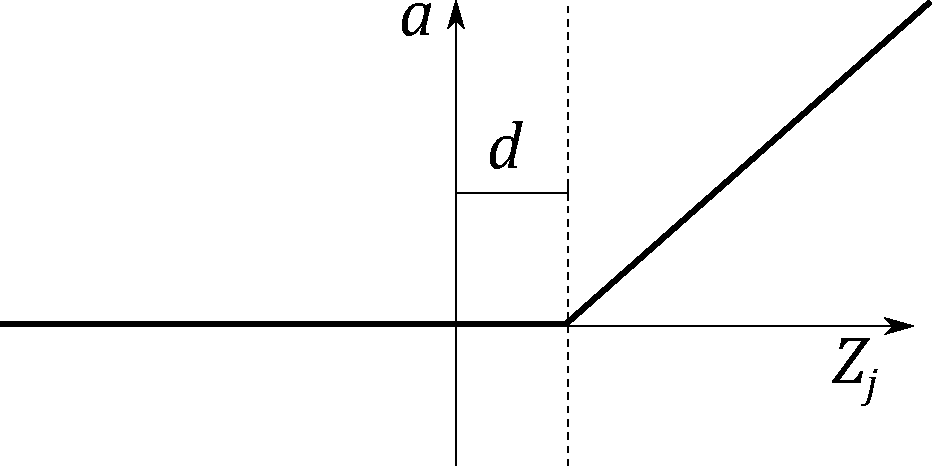
\includegraphics[width=0.5\linewidth]{images/relu.pdf}    

    \caption{In figure captions, explain what the reader is looking at: ``A schematic of the rectifying linear unit, where $a$ is the output amplitude,
    $d$ is a configurable dead-zone, and $Z_j$ is the input signal'', as well as why the reader is looking at this: 
    ``It is notable that there is no activation \emph{at all} below 0, which explains our initial results.'' 
    \textbf{Use vector image formats (.pdf) where possible}. Size figures appropriately, and do not make them over-large or too small to read.
    }

    % use the notation fig:name to cross reference a figure
    \label{fig:relu} 
\end{figure}


\begin{figure}
    \centering
    \begin{subfigure}[b]{0.45\textwidth}
        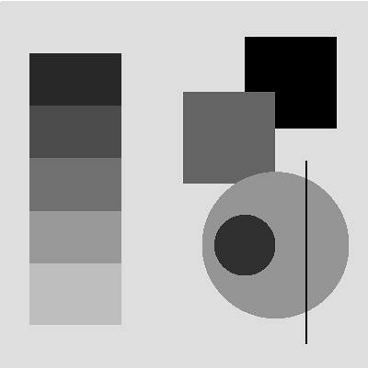
\includegraphics[width=\textwidth]{images/synthetic.png}
        \caption{Synthetic image, black on white.}
        \label{fig:syn1}
    \end{subfigure}
    ~ %add desired spacing between images, e. g. ~, \quad, \qquad, \hfill etc. 
      %(or a blank line to force the subfigure onto a new line)
    \begin{subfigure}[b]{0.45\textwidth}
        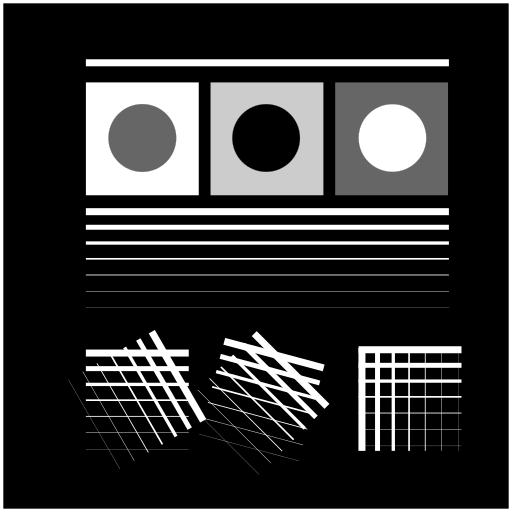
\includegraphics[width=\textwidth]{images/synthetic_2.png}
        \caption{Synthetic image, white on black.}
        \label{fig:syn2}
    \end{subfigure}
    ~ %add desired spacing between images, e. g. ~, \quad, \qquad, \hfill etc. 
    %(or a blank line to force the subfigure onto a new line)    
    \caption{Synthetic test images for edge detection algorithms. \subref{fig:syn1} shows various gray levels that require an adaptive algorithm. \subref{fig:syn2}
    shows more challenging edge detection tests that have crossing lines. Fusing these into full segments typically requires algorithms like the Hough transform.
    This is an example of using subfigures, with \texttt{subref}s in the caption.
    }\label{fig:synthetic}
\end{figure}

\clearpage

\subsection{Equations}

Equations should be typeset correctly and precisely. Make sure you get parenthesis sizing correct, and punctuate equations correctly 
(the comma is important and goes \textit{inside} the equation block). Explain any symbols used clearly if not defined earlier. 

For example, we might define:
\begin{equation}
    \hat{f}(\xi) = \frac{1}{2}\left[ \int_{-\infty}^{\infty} f(x) e^{2\pi i x \xi} \right],
\end{equation}    
where $\hat{f}(\xi)$ is the Fourier transform of the time domain signal $f(x)$.

\subsection{Algorithms}
Algorithms can be set using \texttt{algorithm2e}, as in Algorithm \ref{alg:metropolis}.

% NOTE: line ends are denoted by \; in algorithm2e
\begin{algorithm}
    \DontPrintSemicolon
    \KwData{$f_X(x)$, a probability density function returing the density at $x$.\; $\sigma$ a standard deviation specifying the spread of the proposal distribution.\;
    $x_0$, an initial starting condition.}
    \KwResult{$s=[x_1, x_2, \dots, x_n]$, $n$ samples approximately drawn from a distribution with PDF $f_X(x)$.}
    \Begin{
        $s \longleftarrow []$\;
        $p \longleftarrow f_X(x)$\;
        $i \longleftarrow 0$\;
        \While{$i < n$}
        {
            $x^\prime \longleftarrow \mathcal{N}(x, \sigma^2)$\;
            $p^\prime \longleftarrow f_X(x^\prime)$\;
            $a \longleftarrow \frac{p^\prime}{p}$\;
            $r \longleftarrow U(0,1)$\;
            \If{$r<a$}
            {
                $x \longleftarrow x^\prime$\;
                $p \longleftarrow f_X(x)$\;
                $i \longleftarrow i+1$\;
                append $x$ to $s$\;
            }
        }
    }
    
\caption{The Metropolis-Hastings MCMC algorithm for drawing samples from arbitrary probability distributions, 
specialised for normal proposal distributions $q(x^\prime|x) = \mathcal{N}(x, \sigma^2)$. The symmetry of the normal distribution means the acceptance rule takes the simplified form.}\label{alg:metropolis}
\end{algorithm}

\subsection{Tables}

If you need to include tables, like Table \ref{tab:operators}, use a tool like https://www.tablesgenerator.com/ to generate the table as it is
extremely tedious otherwise. 

\begin{table}[]
    \caption{The standard table of operators in Python, along with their functional equivalents from the \texttt{operator} package. Note that table
    captions go above the table, not below. Do not add additional rules/lines to tables. }\label{tab:operators}
    %\tt 
    \rowcolors{2}{}{gray!3}
    \begin{tabular}{@{}lll@{}}
    %\toprule
    \textbf{Operation}    & \textbf{Syntax}                & \textbf{Function}                            \\ %\midrule % optional rule for header
    Addition              & \texttt{a + b}                          & \texttt{add(a, b)}                                    \\
    Concatenation         & \texttt{seq1 + seq2}                    & \texttt{concat(seq1, seq2)}                           \\
    Containment Test      & \texttt{obj in seq}                     & \texttt{contains(seq, obj)}                           \\
    Division              & \texttt{a / b}                          & \texttt{div(a, b) }  \\
    Division              & \texttt{a / b}                          & \texttt{truediv(a, b) } \\
    Division              & \texttt{a // b}                         & \texttt{floordiv(a, b)}                               \\
    Bitwise And           & \texttt{a \& b}                         & \texttt{and\_(a, b)}                                  \\
    Bitwise Exclusive Or  & \texttt{a \textasciicircum b}           & \texttt{xor(a, b)}                                    \\
    Bitwise Inversion     & \texttt{$\sim$a}                        & \texttt{invert(a)}                                    \\
    Bitwise Or            & \texttt{a | b}                          & \texttt{or\_(a, b)}                                   \\
    Exponentiation        & \texttt{a ** b}                         & \texttt{pow(a, b)}                                    \\
    Identity              & \texttt{a is b}                         & \texttt{is\_(a, b)}                                   \\
    Identity              & \texttt{a is not b}                     & \texttt{is\_not(a, b)}                                \\
    Indexed Assignment    & \texttt{obj{[}k{]} = v}                 & \texttt{setitem(obj, k, v)}                           \\
    Indexed Deletion      & \texttt{del obj{[}k{]}}                 & \texttt{delitem(obj, k)}                              \\
    Indexing              & \texttt{obj{[}k{]}}                     & \texttt{getitem(obj, k)}                              \\
    Left Shift            & \texttt{a \textless{}\textless b}       & \texttt{lshift(a, b)}                                 \\
    Modulo                & \texttt{a \% b}                         & \texttt{mod(a, b)}                                    \\
    Multiplication        & \texttt{a * b}                          & \texttt{mul(a, b)}                                    \\
    Negation (Arithmetic) & \texttt{- a}                            & \texttt{neg(a)}                                       \\
    Negation (Logical)    & \texttt{not a}                          & \texttt{not\_(a)}                                     \\
    Positive              & \texttt{+ a}                            & \texttt{pos(a)}                                       \\
    Right Shift           & \texttt{a \textgreater{}\textgreater b} & \texttt{rshift(a, b)}                                 \\
    Sequence Repetition   & \texttt{seq * i}                        & \texttt{repeat(seq, i)}                               \\
    Slice Assignment      & \texttt{seq{[}i:j{]} = values}          & \texttt{setitem(seq, slice(i, j), values)}            \\
    Slice Deletion        & \texttt{del seq{[}i:j{]}}               & \texttt{delitem(seq, slice(i, j))}                    \\
    Slicing               & \texttt{seq{[}i:j{]}}                   & \texttt{getitem(seq, slice(i, j))}                    \\
    String Formatting     & \texttt{s \% obj}                       & \texttt{mod(s, obj)}                                  \\
    Subtraction           & \texttt{a - b}                          & \texttt{sub(a, b)}                                    \\
    Truth Test            & \texttt{obj}                            & \texttt{truth(obj)}                                   \\
    Ordering              & \texttt{a \textless b}                  & \texttt{lt(a, b)}                                     \\
    Ordering              & \texttt{a \textless{}= b}               & \texttt{le(a, b)}                                     \\
    % \bottomrule
    \end{tabular}
    \end{table}
\subsection{Code}

Avoid putting large blocks of code in the report (more than a page in one block, for example). Use syntax highlighting if possible, as in Listing \ref{lst:callahan}.

\begin{lstlisting}[language=python, float, caption={The algorithm for packing the $3\times 3$ outer-totalistic binary CA successor rule into a 
    $16\times 16\times 16\times 16$ 4 bit lookup table, running an equivalent, notionally 16-state $2\times 2$ CA.}, label=lst:callahan]
    def create_callahan_table(rule="b3s23"):
        """Generate the lookup table for the cells."""        
        s_table = np.zeros((16, 16, 16, 16), dtype=np.uint8)
        birth, survive = parse_rule(rule)

        # generate all 16 bit strings
        for iv in range(65536):
            bv = [(iv >> z) & 1 for z in range(16)]
            a, b, c, d, e, f, g, h, i, j, k, l, m, n, o, p = bv

            # compute next state of the inner 2x2
            nw = apply_rule(f, a, b, c, e, g, i, j, k)
            ne = apply_rule(g, b, c, d, f, h, j, k, l)
            sw = apply_rule(j, e, f, g, i, k, m, n, o)
            se = apply_rule(k, f, g, h, j, l, n, o, p)

            # compute the index of this 4x4
            nw_code = a | (b << 1) | (e << 2) | (f << 3)
            ne_code = c | (d << 1) | (g << 2) | (h << 3)
            sw_code = i | (j << 1) | (m << 2) | (n << 3)
            se_code = k | (l << 1) | (o << 2) | (p << 3)

            # compute the state for the 2x2
            next_code = nw | (ne << 1) | (sw << 2) | (se << 3)

            # get the 4x4 index, and write into the table
            s_table[nw_code, ne_code, sw_code, se_code] = next_code

        return s_table

\end{lstlisting}

%==================================================================================================================================
\chapter{Evaluation} 

In this chapter I will go over the process and results from my two rounds of evaluations.

\section{Process}
The game was tested during the week commencing 23rd January 2023 involving volunteers with a range of Android phones. I set up multiple two player
games that were played around the main building, the cloisters and the surrounding area. Each game lasted 15 minutes where I collected the locations
of the players, their GPS Error and the locations where the players were caught. I also noted down the brand and the model of the phone to analyse
how the game worked with different phones. After playing the game, I would ask my participants to fill in a survey with questions including how
fun the game was to play, whether the connection was stable and what improvements could be made in future iterations. I plan to do two phases
with the second phase set to be done in the week commencing the 6th February 2023.

\section{Results from Phase 1}
\label{phase1}

\subsection{Overview}
For Phase 1 I managed to test the game with 8 participants with a total of 6 games played. Games were either played between me and the participant
or between the two participants. Most of the games went well with the exception of two games where the ranges in errors were higher than my threshold
(I will go into more detail in subsection \ref{phase1errorrange}). I was glad to see that there were no problems with overall connectivity throughout
the duration of the game and that the play tests had an overall positive reception.

\subsection{Strategies}
An interesting thing that came out of this evaluation is the different strategies that some participants made while playing the game. At the beginning
of every game I explained to the participants where some of the best locations to find a GPS shadow would be. With this knowledge most participants
went under the cloisters however one person had a better strategy. They managed to find a route through the University Chapel to the opposite
quadrangle without being detected.

\subsection{Error Ranges}
\label{phase1errorrange}
One of the things that I wanted to see was whether the GNSS accuracies on different phones would be consistent or whether it would vary more.
When I was doing my initial walks finding GNSS Shadows, I only used my personal phone (A Samsung Galaxy S21 FE) to get readings. Figure \ref{fig:galaxys21}
shows the ranges in the Error ratings. From the graph I can see that when this phone is in a relatively open area, the error rate remains constant at around 3.8 meters. There
are only a few peaks throughout the duration of the game. Through experience this only happens when I go into buildings or under bridges and in other areas where GPS performance
is expected to decrease. When developing the game I thought that an error of 6 meters or more would have been the threshold for whether a player was in a GPS Shadow or not as I
assumed that it would be constant for every phone.

When running my game on different phone, I noticed that my assumption that the same range of GPS accuracies were true for all phone was incorrect. Figure \ref{fig:oppo}
shows the Error ranges on an Oppo F19. As you can see from the graph, the range of GPS errors were significantly higher and less consistent than the Samsung phone. I also
noticed that the error would rarely go under the 6 meter threshold. This meant that when this phone was the runner, the chaser was not able to catch or see their location
this led to a major balancing issue. This problem was also found with the Samsung Note 9 (Figure \ref{fig:note9}), with this phone I noticed that the error rate would get
as low as 0 but would rarely be within the 3.8 and 6 range. This would result in their marker making big jumps before becoming invisible again.

From these results I can see that the wide range of android phones would lead to a wide range of GPS sensors. This could be due to many factors, from the amount of satellites
visible to simply the cost of the GNSS sensors. I feel that my original assumption would have been better if I had created the app using iOS, since I would only be developing
for a single phone type. The main conclusion that I decided to make is that I need to find a new way of calculating whether a player is in a shadow or not.
The best way to do this is to consider the median value or the lowest value and then adjust my ranges based on that value.  

\subsection{The Catching Mechanic}
\label{phase1catching}
Another major thing that I wanted to was see whether the catching mechanic (Please see section \ref{catching} for more details on how this works)
was working as intended. I feel that this part of the evaluation had some mixed results. The problems mentioned in section
\ref{phase1errorrange} caused problems to this part of the game as well. Mainly because I had implemented it so that if the
runner was in a GPS Shadow, the catcher could not catch the player. Another thing that I noticed was that when two players
were immediately next to each other, their GPS coordinates would be outside the 5 meter radius. This meant that with a lot of
games there were a few lost seconds while the participants tried to move themselves in order to see if they could catch each other.
My theory as to why this happened would have been due to the mutltipath error. This issue came up the most around the Quadrangles
of the main building. Meanwhile the catching system worked better around the Flagpole.

The problems that I found in regards to the catching mechanic tell me that I need to make two improvements in this area. For one
thing, the catching radius needs to be increased. The 5 meter radius was too small for a catch to be registered in most cases. Therefore
I will look into expanding the radius to 30 meters to account for any multipath problems. The second improvement that I will
make is that I will remove the requirement for the runner to be in a high accuracy area, this is because once when I was a chaser,
I found the runner in a shadow area and I couldn't catch them until we moved into a more open area.




\subsection{Survey Results}
\label{phase1survey}
The main aim for the survey at the end of the evaluation was to get a more opinionated view of how the participants
thought the game went and what improvements they would make. I started by giving them a set of statements and asked
them if they agreed or disagreed with the statements. Table \ref{tab:agree} shows the breakdown of the participents'
responses.

Table \ref{tab:agree} suggests that the overall reaction to the game was positive. For example all 8 participants started
that they enjoyed the game with 3 out of 8 people saying that they really enjoyed it. The survey suggested that the experience
playing the game helped them get a better understanding about how the accuracy of their GPS coordinates can change due to different
factors such as hiding in buildings and under bridges. This had an even stronger response with three quarters of the participants
stating that they strongly agreed that the game educated them on GPS accuracy. However, the last two questions which were
about the game connection and the user interface had a more mixed response. The User Interface had 4 people who had a Neutral
opinion. This was mainly due to the fact that each player had a marker which was the same colour. The connection question
was the only question which had people who said that they disagreed with the statement. This was mainly due to the problems discussed
in sections \ref{phase1errorrange} and \ref{phase1catching}. In future iterations I will have another look at the user interface
and I will look into having multicoloured markers.

At the tail end of the survey I gave each participant a list of potential features that I was thinking of implementing in phase 2.
I asked the participants to rank the following proposed features:

\begin{enumerate}
    \item Limits for how long someone stays in a GPS Shadow
    \item A powerup system which are earned when the player stays in high GPS accuracy areas
    \item The Runner being able to see the Chaser all the time
    \item Having a new winning condition. Something along the lines of a last man standing system
\end{enumerate}

From the responses that I recevied, the most popular feature was to have a limitation on how long someone can stay in a shadow with
5 out of 8 of my participants ranking it first. Surprisingly the least popular feature was letting the Runner see the Chaser all the time.
My guess is that the design for the runner type makes the game more tense if you don't know exactly where the chaser is going to be.
I discussed with the players about the limits on how long someone can stay in a shadow and most people said that it was better to have
a more punishing mechanic than a rewarding one in the form of a powerup system to ensure that the runners don't just stay in the same place.

In the final part of the survey I asked the participants whether they had any further comments or feature ideas. One of the most common
feature ideas brought up in this section was to have a different colour of marker to show who is the chaser and who is the runner. Up to this
point I had just used the generic marker in the Google Maps Jetpack API. Another interesting thing that came up was that I should consider
adding a manual catching mechanic as a potential solution to the problems raised in section \ref{phase1catching}. I feel that this could Be
a good solution but increasing the catch radius would still be an easier solution and would help teach the participants how GPS errors could
come about.

\begin{table}[]
    \centering
    \resizebox{\textwidth}{!}{\begin{tabular}{|l|l|l|l|l|l|}
    \rowcolor[HTML]{9B9B9B} 
    \textbf{Question}                                                                  & \textbf{Strongly Agree} & \textbf{Somewhat Agree} & \textbf{Neutral} & \textbf{Somewhat Disagree} & \textbf{Strongly Disagree} \\ \hline
    The Gameplay was an enjoyable experience                                           & 3                       & 5                       & 0                & 0                          & 0                          \\ \hline
    The game gave me a better sense of awareness as \\to where GPS accuracy can decrease & 6                       & 2                       & 0                & 0                          & 0                         \\ \hline
    The User Interface Displayed information clearly                                   & 2                       & 2                       & 4                & 0                          & 0                          \\ \hline
    The game connection was stable                                                     & 4                       & 2                       & 0                & 2                          & 0                          \\ \hline
    \end{tabular}}
    \caption{At the start of the survey I gave my participants 4 statements and asked them whether they agreed or disagreed with it. This table shows the results of that survey}
    \label{tab:agree}
\end{table}


\section{Guidance}
\begin{itemize}
    \item
        Ask specific questions that address the general problem.
    \item
        Answer them with precise evidence (graphs, numbers, statistical
        analysis, qualitative analysis).
    \item
        Be fair and be scientific.
    \item
        The key thing is to show that you know how to evaluate your work, not
        that your work is the most amazing product ever.
\end{itemize}

\section{Evidence}
Make sure you present your evidence well. Use appropriate visualisations, reporting techniques and statistical analysis, as appropriate.

If you visualise, follow the basic rules, as illustrated in Figure \ref{fig:boxplot}:
\begin{itemize}
\item Label everything correctly (axis, title, units).
\item Caption thoroughly.
\item Reference in text.
\item \textbf{Include appropriate display of uncertainty (e.g. error bars, Box plot)}
\item Minimize clutter.
\end{itemize}



%==================================================================================================================================
\chapter{Conclusion}    
Summarise the whole project for a lazy reader who didn't read the rest (e.g. a prize-awarding committee).
\section{Guidance}
\begin{itemize}
    \item
        Summarise briefly and fairly.
    \item
        You should be addressing the general problem you introduced in the
        Introduction.        
    \item
        Include summary of concrete results (``the new compiler ran 2x
        faster'')
    \item
        Indicate what future work could be done, but remember: \textbf{you
        won't get credit for things you haven't done}.
\end{itemize}

%==================================================================================================================================
%
% 
%==================================================================================================================================
%  APPENDICES  

\begin{appendices}

\chapter{Appendices}

\begin{figure}
    \centering
    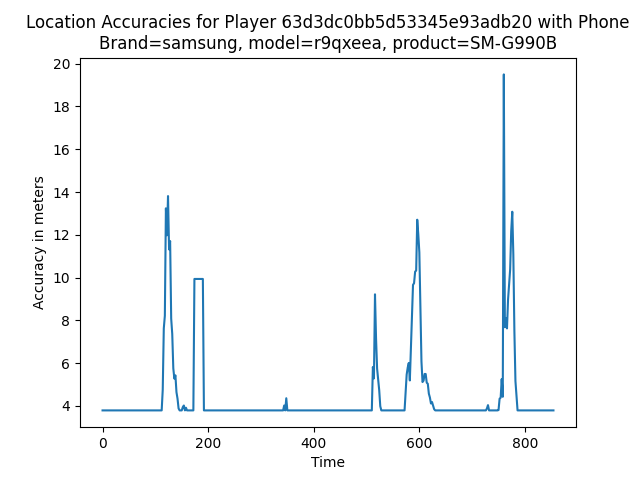
\includegraphics[width=1.0\linewidth]{images/my_phone.png} 
    \caption{The Error ranges found during a game using a Samsung Galaxy S21 FE}
    \label{fig:galaxys21}
\end{figure}
\begin{figure}
    \centering
    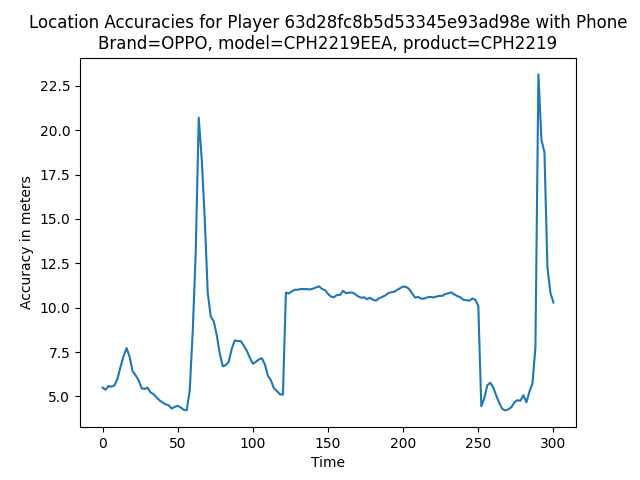
\includegraphics[width=1.0\linewidth]{images/oppo.png}
    \caption{The Error ranges found during a game using an Oppo F19}
    \label{fig:oppo}
\end{figure}
\begin{figure}
    \centering
    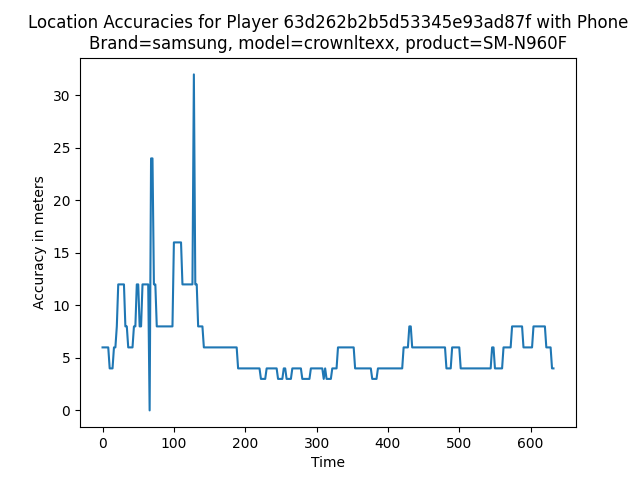
\includegraphics[width=1.0\linewidth]{images/note9.png}
    \caption{The Error ranges found during a game using an Samsung Note 9}
    \label{fig:note9}
\end{figure}

Typical inclusions in the appendices are:

\begin{itemize}
\item
  Copies of ethics approvals (required if obtained)
\item
  Copies of questionnaires etc. used to gather data from subjects.
\item
  Extensive tables or figures that are too bulky to fit in the main body of
  the report, particularly ones that are repetitive and summarised in the body.

\item Outline of the source code (e.g. directory structure), or other architecture documentation like class diagrams.

\item User manuals, and any guides to starting/running the software.

\end{itemize}

\textbf{Don't include your source code in the appendices}. It will be
submitted separately.

\end{appendices}

%==================================================================================================================================
%   BIBLIOGRAPHY   

% The bibliography style is abbrvnat
% The bibliography always appears last, after the appendices.

\bibliographystyle{abbrvnat}

\bibliography{l4proj}

\end{document}
